\chapter*{Introduction}         % ne pas numéroter
\label{chap-introduction}       % étiquette pour renvois
\phantomsection\addcontentsline{toc}{chapter}{\nameref{chap-introduction}} % inclure dans TdM

% Note: This is an un-numbered chapter.

Comminution (grinding) is a particle size reduction process used in mineral processing industries to liberate valuable minerals from ore as part of the concentration process. Figure \ref{fig:process-block-diagram} shows the block diagram of the steps in a typical copper concentration process.

\begin{figure}[htp]
	\centering
	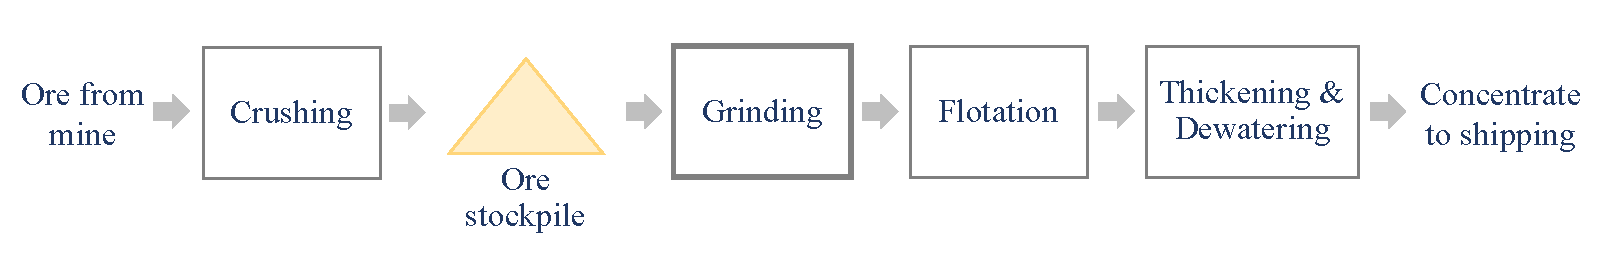
\includegraphics[width=15cm]{images/process_block_diagram.pdf}
	\caption{Processing steps in a copper concentrator} \label{fig:process-block-diagram}
\end{figure}

Effective control and optimization of grinding operations is challenging for a number of reasons---large variations in the properties of the ore feed material, multiple strongly-coupled interacting variables, long time delays, non-linear and time-varying input-output characteristics, process variables that are difficult to measure, and difficulties in identifying process models of actual operations \citep{olivier_dual_2012, gough_sag_2015, le_roux_throughput_2016, aguila-camacho_control_2017}. 

Any input that has a material effect on the state or behaviour of a process and is not manipulatable by the control system is defined as a disturbance. Changes in the properties of the ore feed are a significant problem because they are difficult to measure accurately in real time and their impact on the grinding process and control system can be severe \citep{herbst_optimal_1988, cesar_multivariable_2009, remes_grinding_2010, liu_development_2018}. \cite{powell_applying_2009} summarized the effects of ore variability as follows:

Variable ore $\to$ variable operation $\to$ variable grind $\to$ variable recovery $\to$ lower recovery. 

One of the primary goals of industrial process control is to maintain desired performance in the presence of unmeasured disturbances \citep{astrom_computer_1997}. By detecting and correcting errors in the estimates of the process states, feedback control systems are able to attenuate the effects of disturbances and thus reduce variation in process variables. This is known as the regulation problem and is common in industrial process control applications where the goal is to maintain steady-state operating conditions as closely as possible.

The main benefit of effective regulation is that the process variables remain close to their optimal settings. This is particularly important when there are operating constraints on critical variables that limit the overall process performance. For example, the power output capacity of an electric motor must not be exceeded for safety reasons. In such cases, it may not be possible to reject a disturbance completely. Some variations in the output variables may be unavoidable and thus, ore feed disturbances can have knock-on effects on the downstream process operations (i.e. the separation process). By reducing the magnitude of variability caused by disturbances, the process may be operated closer to the operating constraints on average, yielding a higher performance than would be achievable with high variability, and reduces the magnitude of variations transmitted to downstream processes.

\subsection*{Grinding process}

Tumbling mills are the most common type of grinding equipment used in hard rock grinding applications. The two main types of tumbling mills are the \textit{semi-autogenous} grinding mill (SAG) and the ball mill \citep{king_chapter_2012}. The SAG mill, which is the focus of this research, is used for primary grinding of the \textit{run-of-mine} ore which comes from the mine after crushing. In a SAG mill, large ore particles play a role in the grinding process as well as grinding media (steel balls) added by the operator. Ball mills are typically used in the second stage of grinding to grind oversize particles from the discharge of the SAG mill circuit.

Figure \ref{fig:cause-effect} is a schematic diagram illustrating the main cause-effect relationships in a tumbling mill. Each oval represents an important process variable and the arrows represent the interacting relationships and show the direction of causality. The five variables on the left are the main input variables and the four on the right are the main outputs. Mill contents and breakage rates are internal variables of the process. Here, mill contents has a broad definition encompassing all attributes of the contents, including water, slurry, ore particles, and grinding media.

\begin{figure}[htp]
	\centering
	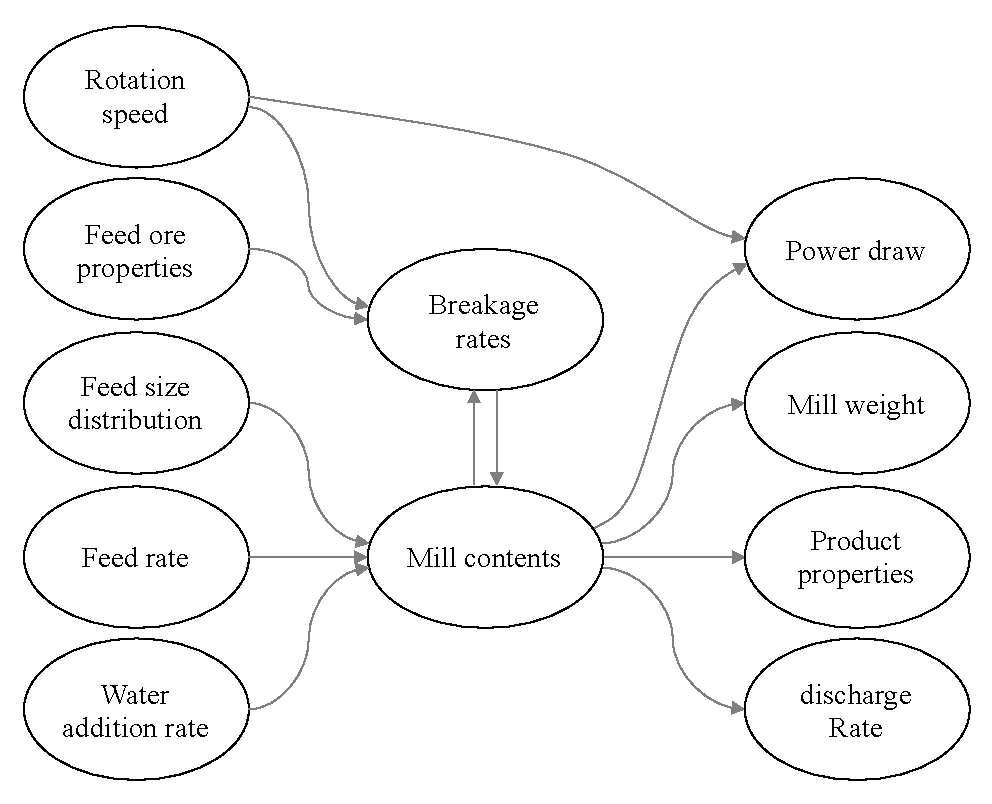
\includegraphics[width=11cm]{images/cause-effect.pdf}
	\caption{Cause and effect diagram} \label{fig:cause-effect}
\end{figure}

\cite{powell_applying_2009} highlighted the interactive (i.e. bi-directional) relationship between mill load and breakage rates and describe how these variables evolve dynamically. A change in ore feed properties, such as a change in hardness or particle sizes, leads to changes in the mill contents, which then affect breakage rates, which have a feedback effect on the evolution of the mill contents. This results in a non-linear response of the output variables which depend on the mill contents.

SAG mills are usually installed in closed-circuit with a classifier. Oversize material that passed out the grate of the mill but does not meet the specification of the classifier is returned to the mill, sometimes via a crusher. This feedback mechanism includes a transport delay which further complicates the dynamic response of the process variables to changes in the inputs.

\subsection*{Grinding process control}

The specific objectives of process control in grinding applications are firstly, to maintain a steady operation and secondly, to optimize the process conditions to achieve maximum operational benefits, for example, maximizing throughput while meeting the product particle size specification \citep{wei_grinding_2009}. Inevitably, trade-offs must be made between competing output variables, such as throughput and product particle size, and between product particle size and power consumption. The focus of this research is to identify and develop methods that facilitate the first objective (i.e. steady operation) given a set of desired operating conditions.

According to a 2007 worldwide survey of grinding circuit operators \citep{wei_grinding_2009}, 63\% reported that the \textit{proportional integral derivative} (PID) control technique was used. \textit{Multivariable control} or \textit{expert systems} were used by 21\%. Less than 10\% reported using \textit{model predictive control} (MPC) or adaptive (self-tuning) control.

The three most commonly controlled variables are the product particle size, the slurry level in the sump, and the sump discharge slurry density. The mill load or filling level also requires some form of control since excursions above or below the normal range can lead to undesirable conditions such as \textit{mill overload} and \textit{freewheeling} \citep{mcclure_overload_2015}. If the load becomes too high, the mill may have to be stopped, resulting in lost production \citep{wei_grinding_2009}.

The main manipulatable variables used for control are the flow rate of water to the sump, the flow rate of water to the mill, the feed rate of solids to the mill, and the discharge flow rate of slurry from the sump. Many modern mills have variable speed drives which allow controlled variation of the rotational speed. However, according to the survey results in 2009, speed is not commonly considered a manipulatable variable.

\cite{najim_adaptive_1995} simulated various adaptive controllers applied to a grinding circuit model with a step disturbance in the ore hardness (represented by a -20\% reduction in breakage rates). The controllers regulate the circulating load and product fineness by manipulating the water addition rate and the fresh ore feed rate.

\cite{pomerleau_survey_2000} simulated various control algorithms applied to a grinding process consisting of a rod mill and a ball mill. The controllers also manipulate the fresh ore and the water feed rates to regulate the product fineness and the circulating load. To compare the performance of the controllers, they simulate a sequence of disturbances to the ore properties---\textit{grindability} and feed size, as well as a change in the number of active cyclones, various and set point changes.

\cite{chen_disturbance_2009} propose a \textit{disturbance observer based} (DOB) control strategy applied to a ball mill grinding circuit model and evaluate its effectiveness in suppressing the effects of a 10\% increase in ore hardness on the product fineness and circulating load.

\cite{olivier_dual_2012} simulate the application of particle filtering to the estimation of both model states and parameters (known as \textit{dual estimation}) of a simulated primary grinding circuit and compare this approach to a simultaneous estimation method. The particle filtering approach is selected because of the non-linearity of the grinding model. They test both approaches in closed loop with decentralized PI controllers.

The first event is the stockpile feeding process of the plant, and the second is the activation/deactivation of secondary grinding circuits.

\cite{le_roux_throughput_2016} simulated a non-linear model-based control architecture to independently control the throughput and product quality of a grinding circuit. To achieve this, they use mill speed as a manipulatable variable, in addition to mill feed rate, water addition, and cyclone feed flow-rate. Their observer also utilises a particle filter to estimate the mill states. However, unlike \cite{olivier_dual_2012}, their observer makes use of measurements that are commonly available in industrial plants, such as mill power and cyclone feed density.

\cite{botha_hybrid_2018} develop and test a hybrid non-linear model predictive controller (NMPC) for a primary grinding mill circuit in which the number of hydro-cyclones (a discrete variable) is used as an additional manipulated variable. They show that this increased controller stability compared to a NMPC without this discrete variable.

\cite{aguila-camacho_control_2017} simulated various types of \textit{fractional order controllers} applied to a grinding circuit model with five manipulatable input variables (fresh ore feed rate, mill inlet feed water rate, sump feed water rate, cyclone feed flow rate, and ball addition rate) and three output variables (mill filling level, sump slurry volume, and product fineness). They also simulated an unmeasured change in the ore feed size distribution.

There is less literature available on the implementation, performance, and benefits of control systems in actual operations. \cite{gough_sag_2015} reports using MPC to control the mill weight, feed rate, and rotation speed of various SAG mills in mines in South America. The controller includes measured disturbances such as pebble recycle rate and ore size distribution as feed forward inputs to improve control. He presents results showing that the MPC is able to reduce the variability in mill weight (84\% reduction in standard deviation) and throughput (55\% reduction in standard deviation) compared to the expert systems that were used in these facilities, resulting in higher production rates.

C.W. Steyn, C. Sandrock (2013) – Benefits of Optimisation and Model Predictive Control on a Fully Autogenous Mill with Variable Speed Application of DMC to an Autogenous (AG) mill. The industrial dynamic matrix controller (DMC) commissioned on the AG mill with a variable speed drive resulted in a 66\% reduction in power and a 40\% reduction in load standard deviation. Anglo American Platinum.
%This reduction in operated variable variability enabled a test campaign where the mill was controlled at various operating regions in order to establish the conditions conducive to the finest product size at a given mill feed rate. Moving the mill operating region from the benchmarked plant to the optimal grind environment and stabilising the mill at this point with the model predictive controller provided an estimated potential recovery increase of 0.32 % (absolute) due to better liberation.

\cite{liu_development_2018} analysed the mineralogical aspects of an operating grinding operation in Western Canada and studied the potential benefits of adjusting mill speed and load to offset changes in mill feed characteristics. However, the analysis is based on a steady-state simulation model and did not look at process control design aspects.


\subsection*{Grinding process observers}

As mentioned above, one of the major obstacles to SAG process control and optimization is the lack of good measurements of critical process variables. For example, breakage rates and the characteristics of the mill contents are not measurable online (i.e. in real time). Of the output variables shown on the right hand side of Figure \ref{fig:cause-effect}, only power draw is directly measurable. Mill weight may be inferred from load sensors or bearing pressure measurements. However, a reliable estimate of the weight of the mill contents is complicated by the fact that the total mill weight includes the weights of the shell and liners, which change over time. Direct measurement of the properties of the discharge of a SAG mill is also impractical due to the properties of the material flow.  Other measurements can be affected by high frequency measurement errors (noise) and others, such as particle size measurements, rely on physical analysis systems which can take minutes to produce new estimates.

For these reasons, process observers which produce reliable online estimates of the unmeasurable variables are an important tool in grinding process control.  As described above, \cite{le_roux_throughput_2016} and others have demonstrated the use of process observers in grinding process control simulations. However, \cite{le_roux_state_2016} went further to determined the identifiability of the internal states and parameters of a simulated SAG mill including the volumetric components of the mill hold-up (water, solids, and fines) and breakage rates. However, they found that measurements of the cyclone discharge flow rate were necessary for identifiability, yet these are not commonly installed in practice.

Outline notes:

\begin{outline}
	%better characterization of these disturbances in real operations → better models → more realistic simulations → better observers → better control and real-time optimization systems/strategies.
	%\1 Many potential benefits: Improve process control performance (reduced variability, disturbance rejection, adaptive control, robustness (i.e. maintain operating conditions within stable region—esp. w.r.t. SAG mill), → improved process performance (throughput, liberation, power consumption, etc.).
	%\1 Use in upstream in the mining operation to help determine the source of variation and identify process improvements.
\end{outline}

Possible references for above:
\begin{outline}
	\1 Papers on observers for mineral processing applications — E.g. 
	\2 Chen et al (2009) - Disturbance Observer Based Multi-Variable Control of Ball Mill Grinding Circuits. (already mentioned in process control above)% chenDisturbanceObserverBased2009
	\2 \cite{le_roux_state_2016} - State and parameter identifiability. 
	\2 Olivier, Huang and Craig (2012) - Dual particle filters for state and parameter estimation.
	\2 LeRoux et al (2016) - State and parameter identifiability, EKF observer.
	\2 LeRoux et al (2016) - Nonlinear observability of grinding mill.
	\2 LeRoux et al (2017) - An EKF observer to estimate semi-autogenous grinding mill hold-ups.
\end{outline}

\section*{Grinding process disturbances}

Continual variability in ore properties such as \textit{hardness}, \textit{competency}, \textit{particle size distribution} (PSD), and \textit{grade} (valuable mineral content) is normal in mining operations due to the geological characteristics of ore bodies. Additional variability is introduced by mining processes such as blasting and crushing, and during material handling operations such as shovelling, trucking, conveying, and storage. Storage systems such as stockpiles, for example, tend to cause segregation of material by particle size, which can result in dramatic changes in the particle size distribution of ore feeding primary grinding if the feed to the stockpile is interrupted \citep{estrada_hybrid_2014}. The nature of such variations will therefore reflect the particular processes and equipment employed at each site. Although they are not random, the complexities of these numerous effects is such that predicting the variations in the properties of ore arriving at the processing plant is extremely difficult.

There is limited available data on actual ore variability in real operations, especially on the dynamic nature of these variations. This may be attributed to the lack of cost-effective measurement technology, the cost of sampling and analysing ore, as well as the commercial sensitivity of such data.

\cite{hahne_ore_2003} carried out tests of ore samples from different points in the production process at a mine in Sweden. The results are used to estimate the influence of feed ore characteristics on grinding performance using a simulation model of the single stage autonomous grinding (AG) circuit. The simulations indicate that the net throughput with a coarse and hard ore is 10\% higher compared to fine and soft ore and that the fine–soft feed results in a coarser particle size distribution of the mill discharge. The amount of coarse material in the feed was found to be the most influential factor. They also found evidence that self-breakage occurs between the mine and the mill since the ore hardness (i.e. its resistance to breakage) increased with the distance from the mining face.

\cite{liu_development_2018} tested samples of different ores from a copper mine in Western Canada as part of a study of the potential benefits of variable speed drives for ball mills. He found that hardness, determined by standard \textit{Bond ball mill work index} (BBWI) tests  (ADD REFERENCE), ranged from 20.2 kWh/t to 27.5 kWh/t. Both these values are in the category `very hard' according to Bueno, et al. (2015). The ore competency, which indicates its resistance to impact breakage, was determined using the JK drop weight test procedure and is expressed in terms of the $A\times{b}$ parameter (Napier-Munn et al., 1996). These were found to range from 29.2 to 39.7, which are categorized as `very hard' and `moderately hard'.

A mineralogical simulation model of the grinding circuits was used to estimate the theoretical maximum possible throughput for each ore type while achieving the desired product specification. They found that the achievable throughput with the least competent ore was 4 times higher than that of the most competent. This illustrates the severe impact that ore properties can have on a grinding operation. However, in the actual operation, different ores are blended to reduce the variation in operating conditions. Liu also estimated the optimal mill speeds to process each ore and found that these ranged from 57.2\% to 64.9\% of critical speed. At these speeds, mill power consumption ranged from 7306 to 9511 kilowatts (a variation of -11\% to +15\% of the average). These results provide a rare insight into the relationship between two important ore properties and grinding process conditions. However, it is unclear how generalisable these results are to other operations.

For the purposes of this work, efforts were made to acquire data on ore properties and operating conditions from other operations. A set of hourly data on ore properties was provided by one mining operation. For commercial reasons, details of the source of this data cannot be disclosed and the data has been normalized and de-trended to remove important features. \textbf{TODO: GET PERMISSION TO SHARE—MAY NOT BE POSSIBLE}. A sample of this adjusted data is shown in Figure X. The two variables are indicators of the ore properties at the feed to the concentrator plant---particle size and hardness. The particle size indicator is based on a real-time measurement---a specialised camera image-based system that provides a dimensionless particle size indication (higher values indicates larger particles). The hardness variable is also a dimensionless indicator produced by a customized operational forecasting model which incorporates data from a variety of sources, including geological data and data from recent drilling activities. The source data is time-delayed according to a model of the flows of material through the mining and ore feed system, therefore this variable is a prediction based on past data inputs and may not reflect current conditions or the actual variability in the feed stream.

There is a limit to what can be deduced from this data but it gives an indication of the possible nature of ore variability in this operation. We can see periods of variation that...  other periods exhibit ... Since the data provided are hourly, they provide no indication of the variations that occur over shorter time-frames, which are of interest in grinding process control design.

%The motivations for this are to 
%\2 realistic disturbance models for simulation
%\2 improved disturbance models for state estimation
%better characterization of these disturbances in real operations → better models → more realistic simulations → better observers → better control and real-time optimization systems/strategies.

This work aims to address the problem of detecting and estimating infrequent, abrupt changes in the ore feed.

Outline notes:

\begin{itemize}
	\item Definition of a disturbance — unmanipulatable inputs to process.
	\item Measured v. unmeasured (and unpredictable)— measured disturbances can be incorporated in a feed-forward control.  Unmeasured disturbances must be estimated in order to reject them.
	\item Importance of considering disturbances in control system design.
	\item Disturbance models and process observers.
	\item \textbf{Should this section go in Method chapter?}
	\item Two categories of disturbances: Infrequent, always-present.
	\item Infrequent disturbances could have significant impact on process and control systems (MacGregor et al).
	\item Standard approaches to system identification do not consider infrequent disturbances (focus on second order properties)
	\item Need for broader range of disturbance model types and ways to incorporate them in control strategies.
\end{itemize}

\section*{Background and objectives}

This work is part of a three-year research and development project by the \textit{Laboratoire d’observation et d’optimisation des procédés} (LOOP) of the University of Laval, with financial support from the Government of Quebec and Nemaska Lithium Corporation. The overall goal of the project is to determine the extent to which technological innovations could transform the current paradigm of mineral processing which is energy intensive and results in significant greenhouse gas emissions. The project consists of two main initiatives:

\begin{enumerate}
	\item Development of dynamic operating models of production units
	\item Development of circuit configurations, process controls, and real time optimization strategies.
\end{enumerate}

Aligned with the second initiative, the specific goals of this research project are to identify or develop disturbance models and observers tailored specifically to the types of disturbances and measurement challenges that exist in real mineral processing operations.

The specific objectives of this research are:

\begin{enumerate}
	\item Propose a model for representing disturbances in mineral processing operations
	\item Propose an observer framework using this model.
\end{enumerate}

\section*{Literature review}

A search of the academic literature was carried out to identify previous work relevant to the project. During this process it became apparent that the number of works related to characterising and modelling disturbances was quite small. With a few exceptions, searches for terms such as `disturbance model' or `disturbance characterisation' tended to result in works dealing with the design of standard stochastic disturbance models, for example \cite{muske_disturbance_2002}, and \cite{pannocchia_robust_2003}, or were focussed mainly on detection and diagnosis of disturbances rather than their simulation or modelling, \cite{thornhill_advances_2007} for example. There is a rich body of work on the subject of fault detection which falls into the second category. In these works, models of the process are used to identify when an \textit{unmodelled} disturbance occurs and to determine its source. However, a typical fault detection algorithm does not have a model of the actual disturbance, therefore its operation is suspended once the disturbance occurs. In contrast, the goal of this work is to identify a model that can be used for state estimation in the presence of disturbances, without interruption.

Some of the exceptions were works on disturbances in specific application domains such as wind power generation, bump disturbances in vehicle suspension systems, and wave disturbances in ship movement control.  In these, researchers developed disturbance models tailored to these applications. For example, \cite{papaefthymiou_mcmc_2008} used a Markov-chain Monte Carlo (MCMC) method to identify and model important characteristics of the wind to generate `synthetic' wind data for the purposes of running realistic dynamic simulations of renewable energy generation systems.

Nevertheless, a small number of research papers were discovered dealing with `realistic disturbances' (loosely defined) occurring in continuous industrial processes. These are also sometimes broadly referred to as `deterministic disturbances' to distinguish them from standard disturbance models based on zero-mean random noise signals (which are truly random in the sense that they are independent and identically-distributed).

\section*{Randomly-occurring deterministic disturbances} \label{RODDs}

In 1984, \cite{macgregor_duality_1984} introduced the concept of the \textit{randomly-occurring deterministic disturbance} (RODD). This is a family of stochastic processes useful for modelling deterministic disturbances commonly encountered in real industrial processes. Three types of RODD process are described by MacGregor and co-workers. One produces infrequently-occurring step changes, another produces a series of ramps, and a third produces a signal consisting of a series of exponential changes. One example of a real-world disturbances that might be represented by these models is that of an unanticipated set-point change made by an operator. Another is an sudden unexpected change to the load on a system. While these disturbances may be deterministic, the key issue is that they are not predictable or measurable by the control system. Therefore, simulating them with a stochastic process driven by a random variable is a reasonable way to emulate their unpredictability for the purposes of control system design.

The structural form of a RODD model is an \textit{autoregressive integrated moving average} (ARIMA) process fed by a special \textit{random shock} signal which has the value 0 most of the time but occasionally, according to a defined probability, has a value sampled from a normal distribution. Depending on the chosen ARIMA process model, this can be used to simulate the different types of RODD disturbances which may act on a process. The details of the RODD model are described in section \ref{subsec-RODD}.

MacGregor and coworkers also showed that the optimal control law derived for a process perturbed by a RODD is no different than that which would be derived for a process subject to a standard stochastic noise.  This is due to the common ARIMA structure of both models and the fact that the expected value (i.e. mean) of the random shock signal is zero as it is for a Gaussian noise. As a result, it is well-suited for use in process control design. For this reason, and in the absence of other alternatives, the RODD disturbance model became a focus of this research project.

\section*{Detection and estimation of RODD disturbances}\label{detection_RODDs}

Traditional filtering methods such as Kalman filters are unable to efficiently estimate RODD disturbances due to the inevitable trade-off that must be made between the ability to track a disturbance when it occurs and the sensitivity to noise \cite{robertson_detection_1995}.

Prior work in the field of process monitoring focused on the problem of fault detection. The disadvantage of these methods was that, once a fault is detected, the estimation process stops, and some sort of corrective action is required before the filters can be restarted. 

In their 1995 paper, Robertson, Kesavan and Lee \cite{robertson_detection_1995} described how unmeasured RODD disturbances perturbing a system can be estimated online using a \textit{multi-model} observer approach that is effective over an extended period of time during which any combination of several disturbances may occur.

Multi-model filtering approaches involve simultaneously computing multiple independent filters with different parameters and then combining the estimates from these filters to produce a better estimate of the system states \cite{jaffer_estimation_1971, buxbaum_recursive_1970, tugnait_detection_1982}.

Unlike the random shock signal defined by MacGregor and co., Robertson and co. use a signal that is sampled from one of two normal distributions, one with a low variance and the other with a much higher variance. This means that the probability density of the shock signal is conditionally Gaussian, whereas the shock signal used by MacGregor and co. has a non-smooth (i.e. degenerate) probability density function.

Since the sequence of past random shocks is not known, each filter's state estimate is calculated assuming a different sequence of past possible shocks. The estimates of some filters are therefore better than those of others, depending on how closely the shock indicator sequences match the disturbances that actually occurred. The overall best estimate of the states is computed by calculating the conditional probabilities of each indicator sequence given the available measurement data, and this estimate is updated recursively each sample period using Bayesian inference.

Due to practical limitations, the optimal multi-model approach cannot be implemented and some kind of approximation is needed to limit the number of filters required. Practical multi-model observers are therefore referred to as \textit{sub-optimal}. Robertson and coworkers propose using a combination of three specific approximations when estimating RODD disturbances.

The first is based on the assumption that correctly estimating the exact timing of RODD disturbances is not important and therefore a filter that assumes a shock occurred within a short period close to the actual occurrence will be adequate. This is based on the observation that when the correction gain of a Kalman filter is increased at time $k$ due to the assumption of a shock occurrence, it tends to remain large for several sample periods thereafter.

The second approximation is based on the assumption that RODD disturbances occur infrequently and it is quite unlikely that two or more shocks occur within a short time period. This further reduces the number of filters required, especially in systems subject to multiple independent disturbances.

The third approximation is referred to as \textit{filter fusion} or the \textit{generalized pseudo-Bayes algorithm} \cite{jaffer_estimation_1971, buxbaum_recursive_1970, tugnait_detection_1982}. This is based on the assumption that only differences in the recent values of the shock indicator sequence affect the state estimates. Therefore, sequences whose last $f$ terms are the same can be combined. In other words, the length of the unique sequences which must be maintained is limited to the previous $f$ sample periods.

Robertson and coworkers present results of simulating their sub-optimal multi-model observer on a 2-input, 2-output, non-linear dynamical system representing a continuous stirred-tank reactor (CSTR) process. They show the estimates produced by the multi-model approach compared with two single extended Kalman filters (EKF) with different noise parameters. The first of the single EKFs is sensitive to the measurement noise and the second is slow to respond to the RODD step disturbances, while the multiple-model observer appears to perform better than either single EKF in the example simulations.

\cite{eriksson_classification_1996} present results of using an adaptive multi-model approach to estimate \textit{infrequently-occurring disturbances}. They utilize the \textit{adaptive forgetting through multiple models} (AFMM) algorithm by \cite{andersson_adaptive_1985}, also previously described by \cite{gustafsson_estimation_1993}. The AFMM algorithm employs a technique called \textit{sequence pruning} \cite{tugnait_detection_1982}, in contrast to the fixed-depth \textit{sequence merging} or \textit{sequence fusion} technique \citep{blom_interacting_1988} used by Robertson and co.

Sequence pruning is the online deletion of sequences that have a low probability given the current measurements. The deleted sequences are replaced by new sequences to represent the possible branches of the most likely sequence at the next sample time. For example, for a system with one infrequently occurring input disturbance, the most likely shock sequence at the next sample time is the shock sequence estimated to be most likely at the current time extended by the addition of a zero to indicate no shock at the next sample time. However, a shock could occur in the next time period. To account for this possibility, a new shock sequence is generated by making a copy of the current most likely sequence and its associated filter and extending it assuming a shock at the next sample time. This new sequence and filter replace the least likely sequence and observer. Thus, the total number of sequences and independent filters that need to be maintained remains constant. Note that in the case of systems with more than one input disturbance, the number of possible branches of the most likely sequence is higher, and therefore a larger number of sequences and filters will be replaced each time step.

There is one restriction to this pruning rule. A sequence created at sample time $k$ cannot be deleted until sample time $k+n_{min}$ where $n_{min}$ is a \textit{minimum life length} parameter. This is necessary because it can take several sample periods before the filter estimates respond to the change and thus the conditional probability of the new sequence is established.

The AFMM algorithm also includes a procedure for online estimation of the measurement noise covariance, using a forgetting factor to control the speed of adaptation of the estimate.\cite{andersson_adaptive_1985}

In Robertson and co., the RODD disturbance model is assumed to be known. This is also the case in Eriksson and Isaksson's paper, however, Eriksson and Isaksson show how the estimation procedure can be extended to discriminate between two possible disturbance hypotheses. They consider the example of determining whether a step disturbance is affecting the output or the input of the process, assuming it is actually present at either but not both simultaneously.

Two sets of Kalman filters are run simultaneously, one set with the infrequently-occurring disturbances modelled at the input of the process and the other set with them modelled at the output. The conditional probabilities of all filter models are calculated every sample time and normalized across both sets of filters.  Thus an online estimate can be made of which disturbance hypothesis is most likely (i.e. an input or output disturbance) as well as an estimate of the magnitude of the disturbance. They provide results from simulated examples and a laboratory experiment to show that the AFMM method correctly estimates the disturbance actually present in each case.

Robertson and Lee published a second paper in 1998. In this paper they list Anderson \cite{andersson_adaptive_1985} among the references on multiple-model algorithms.  However, the approach and sub-optimal method used is essentially the same as in their 1995 paper, with only slightly different terminology used (`infrequently occurring abrupt disturbances' instead of `randomly occurring deterministic disturbances'). 

However, a different non-linear system (a 3-state model of a heptane to toluene aromatization process) is used for the numerical example and, importantly, this time sum-of-squared errors for the parameter estimates are presented averaged over 50 Monte Carlo simulations, so it is easier to compare the different methods. They compare their sub-optimal method with a single EKF and with the generalized pseudo-Bayes (GPB) algorithm (without sub-optimal modifications).

The results show that their sub-optimal filter does 35 percent better than either the EKF or the GPB algorithm. This is simply because their filter has a horizon of 90 minutes (using 22 filters), whereas the standard GPB algorithm has a horizon of only 2 minutes (using 16 filters) so there is not enough time for it to detect changes before the filters are fused.

\section*{Disturbance modelling using hidden Markov models}
\label{hidden_markov_models}

Outline notes:

\begin{itemize}
	\item \textbf{TODO: Much of this we could drop since we did not look at HMM models.}
	\item Wong and Lee proposed a generalized framework for modeling realistic disturbance processes which have both continuous and discrete (i.e. modal) dynamics \citep{wong_disturbance_2007}.
	\item The mode transitions are described by a finite-state \textit{Markov chain}.
	\item The model generating the Markov chain is referred to as a \textit{hidden Markov model} (HMM) because it is unknown and must be inferred from available noisy measurements.
	\item The combined system including discrete and continuous dynamics is termed a \textit{Markov jump linear system} (MJLS) \citep{costa_discrete-time_2005}.
	\item Wong and Lee point out that the application of HMM's and MJLS's in science and engineering is not novel and refer readers to the references in \cite{costa_discrete-time_2005} for prior work by the control community. Nevertheless, they claim that the use of HMMs for disturbance modeling prior to 2007 was limited.
	\item They also note that the RODD disturbance model of Robertson and Lee, and other methods assuming noise inputs described by \textit{mixture-of-Gaussians} (MOG), can be considered special cases of the MJLS.
	\item Unlike Robertson and Lee, who focused on state estimation, Wong and Lee are interested in identification of the model in the presence of non-stationary noise.
	\item Wong and Lee show how the plant and Markov chain parameters may be simultaneously estimated by \textit{maximum likelihood estimation}, specifically, using the expectation maximization (EM) algorithm (see section \ref{mle}).
	\item In their numerical examples, Wong and Lee use a second-order generalized pseudo-Bayesian (GPB2)  method for state estimation \citep{bar-shalom_estimation_1993} (see section \ref{gpba}).
	\item The first example in their 2007 paper, is a disturbance that switches infrequently between a white noise and an integrated white noise.
	\item They compared the prediction errors of a GPB2 observer using the identified MJLS model to those of the best observer with a stationary (i.e. non-switching) model, as well as to those of a GPB2 observer which uses the actual system model.
	\item The 1-step-ahead prediction errors of the GBP2 with the identified model were 26 percent lower than the optimal stationary-model observer and only 7 percent worse than those of the GBP2 with the true model.
	\item These results are averages over 500 simulated realizations, each of 2000 sample periods in length.
	\item The second example is a `soft-sensor' approach for inferential control where the system is subjected to two integrated noise disturbances at the output, each switching between two noise levels with certain probabilities. In this example, the simulation results indicated that the 1-step-ahead prediction errors of the GPB2 observer with the identified model were only 6 percent higher than a GPB2 observer with the true model.
	\item The main limitation of the results presented in the 2007 paper is that they only test the method on systems which switch only in their noise parameters.
	\item The other limitation that they acknowledge, is that the MLE optimization is non-convex and hence may not converge to the global optimum. To mitigate this problem, they chose initial values `suitably close' to the true system parameters.
	\item Although Wong and Lee do not refer to it, it's worth noting that Elliott, Aggoun, and Moore wrote a book on hidden Markov models for estimation and control in 1995 \cite{elliott_hidden_1995}. A central theme of this book is use of so-called \textit{reference probability methods} for optimal estimation and control which they claim are accessible to non-specialists.
	\item Reference probability methods involve a change of probability measure (they are also known as the \textit{measure change approach}) which allows the original estimation and control problem to be reformulated so that well-known results for \textit{identically and independently distributed} (i.i.d.) random variables can be applied, thus simplifying the analysis and the computational complexity. \emph{TODO}: where does this approach fit in with the other concepts (e.g. in Costa's book) and is it still relevant today?
	\item Hybrid systems (e.g. 1999 book by Sworder and Boyd on estimation of hybrid systems)
	\item Discrete time Markov Jump Linear systems (MJLS) (Costa 2005 book)
	\item Problems of observability and Identifiability of Jump Linear Systems (Vidal et al. 2002).
	\item Bemporad on identification of switching systems - e.g. mixed-integer programming (2001), jump models (2018), jump Box-Jenkins model (2020)
	\item Other estimation methods—particle filtering (Arulampalam, 2002 tutorial).
	\item Control of processes subject to intermittent disturbances. MacGregor - duality, Costa book (2005), Wong and Lee efforts (2007), (2009), (2020), (2011), Camacho et al. ()2010).
	\item TODO: Explain field of sequential Monte Carlo techniques (includes particle filtering, EM, etc.).  Holistic view.
\end{itemize}

\section*{The hidden Markov model for process control}
\label{hmm_control}

Outline notes:

\begin{itemize}
	\item \textbf{TODO: Should I include this summary of application of HMM to process control?}
	\item Wong and Lee's 2009 paper \cite{wong_realistic_2009} goes further than their 2007 paper \cite{wong_disturbance_2007} by demonstrating how the proposed HMM-based disturbance framework can be integrated into existing model-based control formulations.
	\item After introducing the HMM framework again, they present 3 numerical examples demonstrating the use of the framework in process control methods and applications, including one to mitigate the impact of highly-varying feed streams entering an ethanol-producing bioreactor.
	\item They provide only a brief review of system identification methods for Markov jump systems and note that it was still an open area of research at the time.
	\item Due to the difficulties of MJLS identification, they bypass the issue in this paper, and assume that the system, noise and Markov parameters are available.
	\item As in the 2007 paper, they use the second order Generalized Pseudo-Bayesian algorithm (GPB2) developed by Bar-Shalom \cite{bar-shalom_estimation_1993}.
	\item Although they don't use it, Wong and Lee also mention the interacting multiple model (IMM) algorithm which they say has a similar performance as GPB2 but at the computational cost of GBP1 \cite{wong_realistic_2009}. \textbf{TODO}: Need to see where this fits in.
	\item The GPB2 algorithm is a recursive estimation scheme, characterized by `branching' and `merging' steps. Wong and Lee provide a simple numerical example of the algorithm including plots of the output and state estimates. Refer to Fig. 3 in \cite{wong_realistic_2009}.
	\item The first of the three examples in the 2009 paper demonstrates the use of the HMM disturbance framework for offset-free linear model predictive control (LMPC) on a single-input, single-output system.
	\item Four simulation scenarios are considered for this example: low input noise compared to output noise, high input noise compared to output noise, similar input and output noise levels, and switching levels of input and output noise (all simulations were run with negligible measurement noise).
	\item In order to investigate model-plant mismtch, four different model-predictive controller/estimator pairs were constructed: one with an output disturbance only, one with only an input disturbance, one with both input and output disturbances, and the fourth with switching behaviour (using the GPB2 estimator).
	\item For each of the four simulation scenarios, 500 realizations, each of duration 500 sample periods, were run and a controller coupled with a time-varying Kalman filter assuming perfect knowledge of the true simulation regime was simulated for benchmarking purposes.
	\item Each controller is evaluated by the average ratio of its squared-tracking error and that of the benchmarking controller/estimator.
	\item The simulation results show that the proposed MPC designed with the HMM model and GPB2 estimator yields the best performance over all simulation scenarios.
	\item Example 2 demonstrates the closed-loop performance of the HMM control approach in detecting and rejecting deterministic step changes.
	\item The controller's performance is compared to a well-tuned controller based on the \textit{integrated white noise} (IWN) approach to rejecting such perturbations.
	\item The results show that the HMM framework achieves an increase of only 6 percent in the error when compared to the ideal full-feedback controller, and yields better performance than a well-tuned IWN-based estimator.
	\item The third example concerns the control of a nonlinear ethanol fermentation process simulation model where the HMM framework is used to represent the highly-varying nature of the feed concentrations.
	\item The glucose concentrations entering the process are modelled as fluctuating among several mean levels (low, mid and high) and the transitions are governed by a Markov chain.  The problem is such that the regime transitions are infrequent since changes in feed type/quality tend to occur on time scales that are longer than that of the plant’s dynamics.
	\item A \textit{sequentially-linearized MPC}, which is a computationally attractive alternative to a full non-linear MPC implementation \cite{lee_extended_1994}, is used to evaluate the closed-loop performance.
	\item The effect of different types of feedback is compared: Full state feedback including the Markov decision variable; Markov decision variable and output feedback only, and output feedback only (corrupted by measurement noise).
	\item As in the previous example, a controller/estimator pair that operates on the common assumption that the disturbance is integrated white noise (IWN) is used as a benchmark.
	\item Not surprisingly, the results indicate that the amount of information available to the controller determines the closed-loop performance, especially, knowledge of the Markov state trajectory. However, all three HMM-based approaches are better than the benchmark closed-loop system relying on the output measurements only.
	\item The authors concluded that the benefits of an HMM-based disturbance framework are ``most immediately reaped" by incorporating them within existing control methodologies such as MPC, as opposed to the optimal control policies developed specifically for Markov jump systems, such as those described in \cite{costa_discrete-time_2005}.
	\item Finally, they stated that the development of systematic model identification methods and more robust control algorithms for Markov jump systems was the focus of their ongoing research.
	\item In 2011, Wong and Lee published a conference paper on the HMM framework for disturbance modelling in which they present the framework again. Again they use the GPB2 algorithm for sub-optimal filtering and present results of two numerical examples. One for state estimation with abruptly changing feed conditions for a `second generation' bioethanol fermentor, and the second for the case of tracking stiction in a mechanical valve, which is a non-trivial detection problem.
	\item As in the previous papers, the results show better performance for the HMM-based approaches.
\end{itemize}


\section*{Contributions of this research}

The main contributions of this research are:

\begin{enumerate}
	\item A review of academic literature pertaining to `realistic' disturbance modelling and state estimation in industrial process operations.
	\item Evaluation of the capabilities of two multi-model observer algorithms by simulations in MATLAB.
	\item Evaluation of the performance of one of the multi-model observers applied to state estimation of a simulated grinding process.
	\item Evaluation of the benefits of one of the multi-model observers as part of a simulated control system applied to the simulated grinding process.
	\item T.b.d.: A case study of the application of model identification techniques to characterise disturbances using data from a real industrial operation.
\end{enumerate}

\section*{Organisation of this report}

Chapter 1 describes the methods used in the research including the disturbance model, the observer designs and the grinding simulation model used for evaluation of one observer.  Chapter 2 describes the simulations carried out to demonstrate the disturbance model and to evaluate the performance of the observers (TODO: And to estimate the potential benefits?). Chapter 3 describes simulations carried out to test some of the possible methods to identify and characterise disturbances from measurement data.
